\section{Population and Sample, Parameters and Statistics}

Data collection is a crucially important step in Statistics. We use the collected and observed sample to make statements about a much larger set - the population.

\begin{definition}{}
  A \textbf{population} consists of all units of interest. Any numerical characteristic of a population is a \textbf{parameter}. A \textbf{sample} consists of observed units collected from the population. It is used to make statements about the population. Any function of a sample is called \textbf{statistic}.
\end{definition}

In real problems, we would like to make statements about the population. To compute probabilities, expectations, and make optimal decisions under uncertainty, we need to know the population \textit{parameters}. However, the only way to know these parameters is to measure the entire population, i.e., to conduct a census.

Instead of a census, we may \textit{collect data in a form of a random sample from a population} (Figure 1). This is our data. We can measure them, perform calculations, and estimate the unknown parameters of the population up to a certain measurable degree of accuracy.

\begin{figure}[ht]
  \centering
  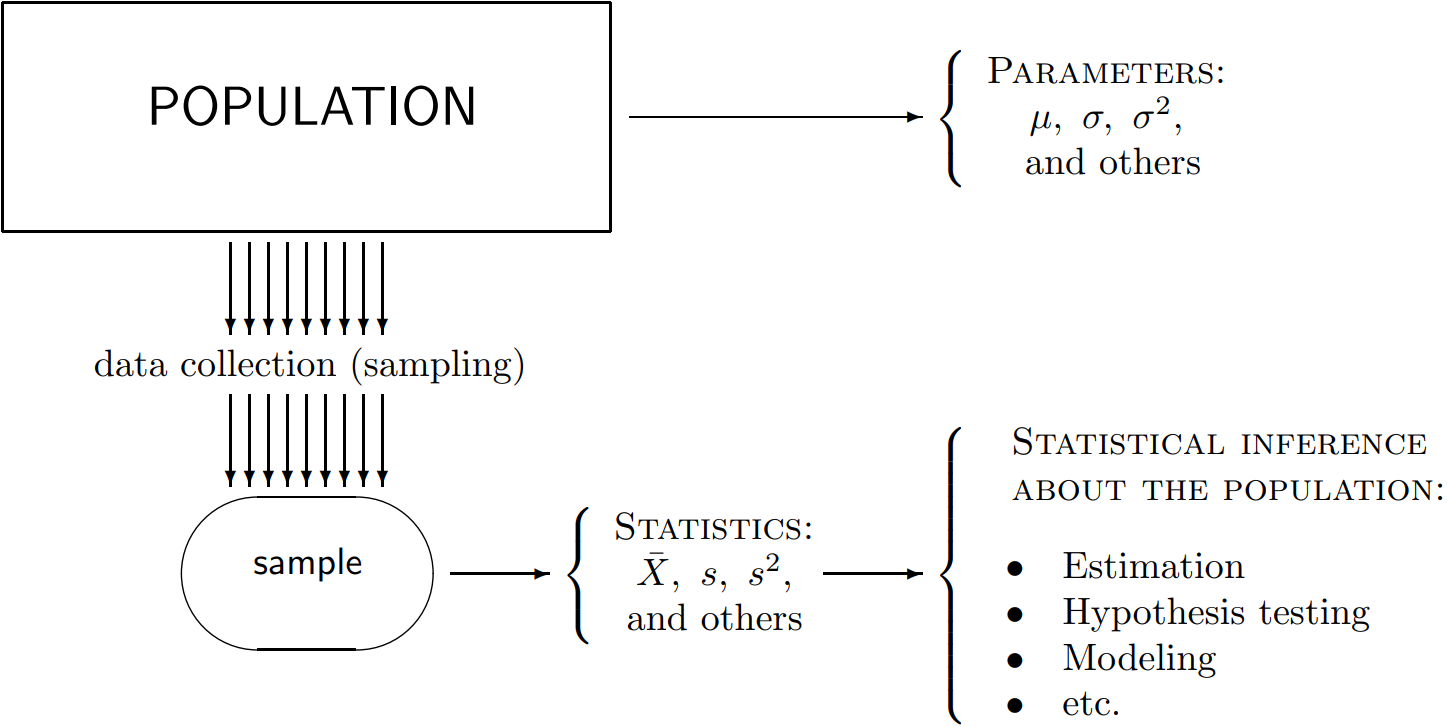
\includegraphics[width=.7\textwidth]{img/fig8-1.png}
  \caption{\textit{Population parameters and sample statistics.}}
\end{figure}

A sample may sometimes give a rather misleading information about the population although this happens with a low probability. \textit{Sampling errors cannot be excluded}.

\subsection{Sampling and Non-sampling Errors}

Sampling and non-sampling errors refer to any discrepancy between a collected sample and a whole population.
\begin{itemize}
  \item \textbf{Sampling errors} are caused by the mere fact that \textit{only a sample, a portion of a population, is observed}. For most of reasonable statistical procedures, \textit{sampling errors decrease (and converge to zero) as the sample size increases}.
  \item \textbf{Non-sampling errors} are caused by \textit{inappropriate sampling schemes or wrong statistical techniques}. Often no wise statistical techniques can rescue a poorly collected sample of data.
\end{itemize}

\noindent \textit{\textbf{Note:} Check the examples 8.1-8.5 in the textbook.}

We will focus on \textit{simple random sampling}, which is one way to avoid non-sampling errors.

\begin{definition}{}
  \textbf{Simple random sampling} is a sampling design where units are collected from the entire population independently of each other, all being equally likely to be sampled.
\end{definition}

Observations collected by means of a simple random sampling design are \textbf{iid} (\textit{independent, identically distributed}) random variables.

\begin{example}{}
  To evaluate its customers' satisfaction, a bank makes a list of all the accounts. A Monte Carlo method is used to choose a random number between 1 and $N$, where $N$ is the total number of bank accounts. Say, we generate a Uniform$(0,N)$ variable $X$ and sample an account number $\left\lceil X \right\rceil$ from the list. Similarly, we choose the second account, uniformly distributed among the remaining $N - 1$ accounts, etc., until we get a sample of the desired size $n$. This is a simple random sample.
\end{example}
